\documentclass{book}
\usepackage{graphicx}
\usepackage{caption}
\usepackage{subcaption}
\usepackage{float}
\usepackage{amsmath}
\usepackage{seqsplit}
\usepackage{tikz}
\usepackage{pgfplots}
\newcommand\longnumber[2]{%
    \begin{minipage}{#1}
    \seqsplit{#2}
    \end{minipage}
    }
\graphicspath{ {images/} }
\begin{document}
\title{A History of Human Communication}
\author{Dan Auerbach}
\date{2015}
\maketitle

\part{The Telegraph}

Some grabbing anecdote...

\chapter{Symbols, Semaphores, and the Optical Telegraph}

If I tell you to envision a telegraph, you may draw up in your mind some electrical apparatus. You are likely not that far off the mark, and we will soon learn the inner workings of Samuel Morse's electrical telegraph which wired the Victorian world, a precursor to the modern Internet. But the word ``telegraph'' was coined long before Morse ever fiddled with electricity, and was originally used to describe a system for conveying information quickly over long distances that involved no wires or electricity at all. Instead, this \emph{optical telegraph} was based on an ancient paradigm: ordinary sight.

\section{The First Telecommunication Network}

Suppose you decide to play a game of catch with your friend Mary. After throwing back and forth a little, the inner athlete in Mary takes over and she decides just throwing the ball around is too boring -- she wants to practice some drills.

You're too far apart to yell at each other, so she waves you over. Soon she is excitedly describing her workout plan to you: for each throw, she is going to tell you for each throw whether she wants a high ball, or a fast line drive ball thrown hard, and your job is to deliver these balls. The point of the exercise isn't to surprise her -- she prefers to know what is coming -- but to deliver the throws she wants as accurately as possible.

You grumble to yourself about Mary's inability to just have fun without making activities so competitive, but know that it would be futile to resist. And besides, you have a much more practical question in front of you: how is she going to indicate if she wants a high ball or a low ball? After all, she's far enough away that shouting is no use. The two of you briefly consider having her hold up one finger for a high ball, and two for a low ball, but quickly realize it will be hard to discern the number of fingers she's holding up from a distance.

After a few seconds, you find a good system. She will raise her right arm straight up in indicate that she wants a high ball thrown, and will put her right arm straight out sideways for a low ball:

\begin{figure}[H]
\centering
\captionsetup{labelformat=empty}
\begin{minipage}{.4\textwidth}
  \centering
  
\includegraphics[width=.3\linewidth]{stick-figure-arm-raised}
  \captionof{figure}{High ball}
  \label{fig:test1}
\end{minipage}%
\begin{minipage}{.4\textwidth}
  \centering
  
\includegraphics[width=.3\linewidth]{stick-figure-arm-sideways}
  \captionof{figure}{Low ball}
  \label{fig:test2}
\end{minipage}
\end{figure}

This works like a charm. Mary chooses the ball she wants, and gets to practice her catching, and you have to admit that it is kind of fun to practice particular types of throws instead of just generally playing catch.

Now, just as you are getting into a rhythm, Mary waves you over again, and your suspicions are quickly vindicated as she explains that she now wants to be able to signal one of \emph{six} different types of throws for you to deliver to her. After some grumbling, you give in and find yourself again faced with the task of coming up with a system for distinguishing the throws from one another without being able to communicate verbally.

The arm-based signaling system was working pretty well, so you decide to extend it, this time using two arms instead of one:

\begin{figure}[H]
\centering

\includegraphics{stick-figure-six-positions-simplified}
\end{figure}

It takes a little getting used to, but you pick up the system and once again settle into a rhythm, having hopefully satiated your throwing partner's lust for pushing her body to the limit. You then start to wonder if you could extend your system even further. Is there a limit to how much information you can convey with just two arms?

After thinking through it a bit more, you realize that if you could represent every letter of the alphabet via a different set of arm positions, then you could signal letters, one at a time, and communicate entire sentences back and forth. It's not too difficult to come up with such a system:

\begin{figure}[H]
\centering
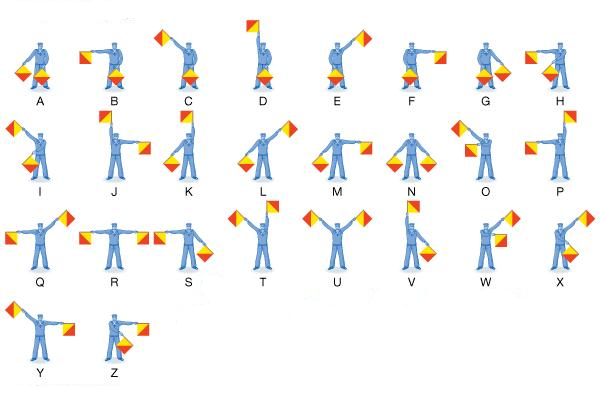
\includegraphics[width=0.9\linewidth]{semaphore_flags}
\end{figure}

Here we display one possible system where the person signalling holds flags for extra emphasis so that the arm positions can be seen from far away.

Using this system, you could compose a message (``hey Mary, let's stop being so intense when we play catch''), and pass that message to Mary encoded via your arm signaling system, who in turn could decode it and in doing so receive the message.

This system is an example of what we can call a \emph{semaphore system} of communication. It may not seem all that groundbreaking. After all, a lot of the decisions were arbitrary and we came up with them in a pretty ad hoc fashion. And it may not seem all that useful for your game of catch; it would certainly be faster to jog 25 yards towards her and speak a full sentence aloud than it would be to try to spell out dozens of letters via arm positions.

But is there any way for us to extend the essence of this idea to quickly transfer information across dozens or even hundreds of miles? 

This question was on the mind of a twentysomething in Paris way back in the 1780s. His name was Claude Chappe, and though he was not an expert on communication systems, he experimented furiously and through trial and error was able to devise a system that could be made to work for sending messages hundreds of miles much more quickly than human beings had ever been able to communicate messages before.

\subsection{The Chappe system}

There were two key extensions to our idea above that Chappe employed in order to mold the ideas we just explored into a useful communication system.

First, instead of using human arms, there would have to be big mechanical ones raised high on a tower so that it could be seen from as far away as possible. In particular, there were two arms both connected to a large cross arm. Such a tower looked something like this:

\begin{figure}[H]
\centering
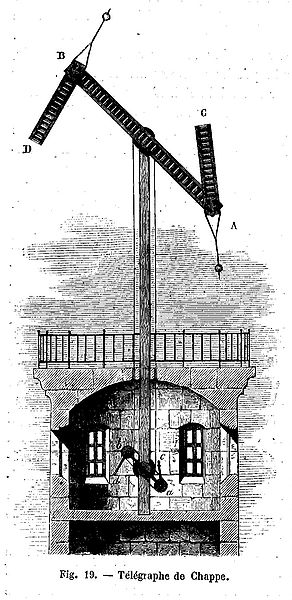
\includegraphics[width=0.3\linewidth]{chappe_tower}
\end{figure}

This obelisk was given the name telegraph, which we could translate as ``distant writer.'' Similar to how we used human arms when experimenting with communication earlier, the arms of the tower could be given many different positions, each corresponding to a different letter or phrase. The advantage of the mechanical arms over human ones, of course, is that the arms on the tower are much larger and hence can be seen from further away.

Second, for Chappe's system to work, there would have to be a vast network of such towers, each 10 to 20 miles apart, which was just close enough for each tower to see the next with the aid of a telescope. While there was not anything particularly novel about Chappe's system, the combination of his perseverance and fortuitous timing made this possible. In fact, the technology behind the Chappe system was well known for quite some time -- Robert Hooke had devised a similar system over a hundred years earlier in England in 1684, but it was never put into practice.

Why did Chappe's vision materialize whereas Hooke's did not? In both cases, government funding was necessary to finance the project, given large infrastructure costs associated with building and maintaining towers. But when Chappe was lobbying the French government in 1792, it was an especially tumultuous period in French history: the first phase of the French revolution had begun only a couple of years earlier, and the French Revolutionary Wars were beginning to take place. Given this backdrop of extreme change and military conflict, the value of facilitating fast information flow became apparent and Chappe's vision was embraced.

With government backing, the first line between Paris and the town of Lille was completed in 1792 and within a few years, this telegraph network spanned much of France:

\begin{figure}[H]
\centering
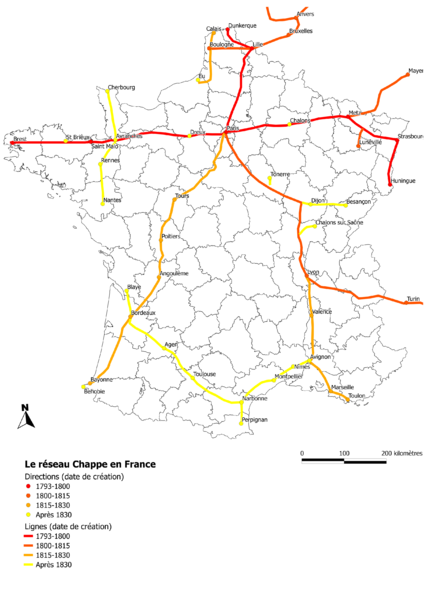
\includegraphics[width=0.5\linewidth]{chappe_network}
\end{figure}

This was the world's first telecommunications (``distant communication'') network, and it required no wires at all. 

The network in France was copied in other countries, as telegraph towers started appearing all over. Indeed, if you live in a city, you may have a neighborhood nearby called something like \emph{telegraph hill}; this name is derived from the hills upon which optical telegraphs were placed. 

The optical telegraph was the first time in history that messages could be delivered many miles away in a relatively short amount of time, and for the next half century, this was the only systematic method for doing so.

\section{A System of Lights}

Chappe's system is one way to communicate effectively at a distance, but are there more practical systems that we might employ for this purpose that make use of visual aids?

Suppose that your football-playing friend Mary lives several miles away on a hill which is clearly visible from your house. Just after your game of ``catch,'' as you are about to part ways, Mary extends you an open invitation to dinner for being such an excellent quarterback. She tells you to come any night that you would like -- how nice of her!

Unfortunately, there is a catch. Mary prefers a quiet life and so has no phone or Internet connection. She assures you that she will be reliably cooking every night, and that if you show up around 8 o'clock in the evening, you will be able to enjoy whatever she has prepared and there is no need to let her know in advance that you'll be joining.

But alas, you are a vegetarian, and Mary sometimes likes to cook meat. While you enjoy Mary's company, it's definitely not worth a forty five minute hike to her house unless you know Mary has cooked a meal you can enjoy.

How can Mary communicate to you so that you know whether or not to come?

You immediately think of Chappe and his two-armed tower (having studied up on your phone after your football game sparked your curiosity about communication systems) but quickly realize that the feasibility of building and placing such a tower on Mary's roof is far-fetched, to say the least.

And then just as you are about to give up, Mary remembers that she has a huge bright light on her roof that when turned on is visible to you from your house. If she is cooking a meal with meat, she will shine the light and leave it on all evening. That way you will know that if you see the light on, you should avoid coming over.

How does this simple communication system work? There are only two possible configurations for the light: on or off. Let's name the light being on as $1$ and the light being off as $0$:

\begin{figure}[H]
\centering
\begin{minipage}{.5\textwidth}
  \centering
  
\includegraphics[width=.5\linewidth]{house_on_hill_0}
  \captionof{figure}{``0'' (light off)}
\end{minipage}%
\begin{minipage}{.5\textwidth}
  \centering
  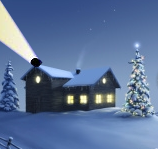
\includegraphics[width=.5\linewidth]{house_on_hill_1}
  \captionof{figure}{``1'' (light on)}
\end{minipage}
\end{figure}

We can write our simple system as follows:

\begin{align*}
	0&: \text{no meat} \\
	1&: \text{meat}
\end{align*}

This works great as a system for Mary to message you about dinner, but now there's a twist -- you have a mutual friend Fred who cannot consume dairy, but does enjoy meat. In order for the system to work for both you and Fred, Mary now has to broadcast whether or not the meal being prepared that night contains meat (for you) and whether or not the meal contains dairy (for Fred). The solution is easy enough: Mary installs a second bright light, clearly distinguishable from the first. The second light is on if and only if the meal has dairy. So now when you or Fred look on Mary's house on the hill there are 4 possible configurations:

\begin{align*}
	00&: \text{no meat, no dairy} \\
	01&: \text{no meat, dairy} \\
	10&: \text{meat, no dairy} \\
	11&: \text{meat, dairy}
\end{align*}

\begin{figure}[H]
\captionsetup{labelformat=empty}
\centering
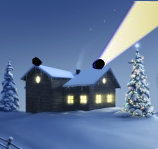
\includegraphics[width=0.25\linewidth]{house_on_hill_01}
\captionof{figure}{Example of one possible configuration ``01'' (first light off, second light on)}
\end{figure}

As we've seen, by combining 2 lights we can display 4 possible configurations. What happens when we add another friend to the mix, with an aversion to gluten? With 3 lights, how many possible configurations can we display? For each of the possible configurations we've already listed above, the third light can either be on or off, effectively doubling the number of possible configurations.

\begin{align*}
	0\quad00&: \text{no gluten, no meat, no dairy} \\
	0\quad 01&: \text{no gluten, no meat, dairy} \\
	0\quad 10&: \text{no gluten, meat, no dairy} \\
	0\quad 11&: \text{no gluten, meat, dairy} \\
          \\
	1\quad 00&: \text{gluten, no meat, no dairy} \\
	1\quad 01&: \text{gluten, no meat, dairy} \\
	1\quad 10&: \text{gluten, meat, no dairy} \\
	1\quad 11&: \text{gluten, meat, dairy}
\end{align*}

Hopefully you are starting to see a pattern. With every light we add, we double the number of possible configurations that can be displayed.

\begin{align*}
1 \text{ light} &= 2 \text{ configurations} \\
2 \text{ lights} &= 2*2 = 4 \text{ configurations} \\
3 \text{ lights} &= 2*2*2 = 8 \text{ configurations} \\
4 \text{ lights} &= 2*2*2*2 = 16 \text{ configurations} \\
5 \text{ lights} &= 2*2*2*2*2 = 32 \text{ configurations} \\
6 \text{ lights} &= 2*2*2*2*2*2 = 64 \text{ configurations} \\
7 \text{ lights} &= 2*2*2*2*2*2*2 = 128 \text{ configurations} \\
8 \text{ lights} &= 2*2*2*2*2*2*2*2 = 256 \text{ configurations} \\
9 \text{ lights} &= 2*2*2*2*2*2*2*2*2 = 512 \text{ configurations} \\
&\text{etc}
\end{align*}

Written more concisely, we have just seen that if we have some number $n$ lights, then we can display $2^n$ possible configurations.

Here the letter '$n$' is a variable. It could stand for $1$ or $4$ or $442424323$. And the notation above refers to exponentiation -- it's just a shorthand way of saying 2 multiplied by itself $n$ times:

\[ 2^n = \underbrace{2*2*2*...* 2}_{\text{n times}}\]

But let's back track a moment to notice that something remarkable happens once we get up to 5 lights. We can now convey one of $2^5 = 2*2*2*2*2 = 32$ possible configurations, which means we have enough information to display each letter of the 26-character alphabet, with some room left over for spaces, commas, periods, and a few other important characters.

And since a single 5-light set can display a single letter (or space, or period), then what happens if we string together multiple sets of 5-lights? You can imagine, perhaps, several 5-light sets on top of Mary's house, although the analogy will soon start to strain the bounds of realism given how difficult it would be to tell each light from the next. (And being able to distinguish each individual light is critical -- knowing that 4 lights are on out of 10 gives you far less information than knowing \emph{which} four of the ten lights is on.)

With 105 sets of 5 lights ($105*5=525$ lights total), Mary could convey this entire 105-character sentence.

Another remarkable thing happens when we start adding lights to our communication system: the number of possible configurations quickly gets astronomically large rather quickly.

For example, with 27 lights, Mary can display... 

\[ \underbrace{2 * 2 * ... * 2}_{27 times} = 2^{27} = 134217728\] 

...over 134 million possible configurations!

Consider the 525 lights that could be used to convey the self-referential sentence above. The number of possible configurations that can be displayed with this many lights is 2 multiplied by itself 525 times, or $2^{525}$.

This is greater than $10^{158}$, or a one followed by 158 zeroes: \\

\longnumber{4in}{1000000000000000000000000000000000000000000000000000000000000000000000000000000000000000000000000000000000000000000000000000000000000000000000000000000000000000} \\

To get a sense of how large this number is, suppose we were to try to cycle through every possible configuration of our 525 lights, displaying them all one configuration at a time. For example, all the lights being on is one possible configuration, so this would appear somewhere when we cycle through. Another possible configuration is Light \#411 being on, Light \#21 being on, and the rest being off. A third example of a possible configuration is all lights being on except for Light \#45.

We have described three possible configurations. Of course there are many, many more. You might guess that with enough painstakingly tedious work one could write down all of the possible configurations as strings of 0s and 1s for our 525 light system, just as we wrote down all of the 8 possibilities for a 3 light system. After all, writing down a few of the possible configurations doesn't seem so bad, since each possible configuration only requires 525 characters. Once we have them written down, you might think programming a computer to cycle through them wouldn't be too hard either.

However, with a little arithmetic, we can see just how clearly impossible it would be to list or cycle through displaying all of the configurations.

Suppose ``Mary'' was actually a cluster of supercomputers. Let's suppose each computer can rotate through a hundred thousand trillion ($10^{17}$) possible configurations per second. That is far more powerful than the world's most powerful supercomputer as of the writing of this text in 2015. And suppose further that there were a trillion computers in the cluster -- this is more computers than we have on the planet, even if you count phones, tablets, laptops, servers, smartcollars for dogs -- everything. But in our extreme hypothetical we have a trillion computers each counting a hundred thousand trillion possibilities per second.

To multiple two exponential numbers together, you merely add their exponents: 

\[10^{12} * 10^{17} = \underbrace{(10*10... *10)}_{12 times} * \underbrace{(10*10*... * 10)}_{17 times} = \underbrace{(10*10*...10)}_{29 times} = 10^{29}.\]

So that means the cluster is able to count $10^{29}$ configurations per second.

There are 60 seconds in a minute, and 60 minutes in an hour, and 24 hours in a day, and 365 days in a year. So that mean that our ``Mary'' cluster counts $10^29 * 60 * 60 * 24 * 365 = 3.1536*10^{36}$ configurations per year.

How many years would it take for our ``Mary'' supercluster to finish this task? In order to compute that, we must take the roughly $10^{158}$ total possible configurations and divide it by the $10^{36}$ possibilities displayed per year. (And dividing two exponential numbers with the same base in involves subtracting the exponents -- try it). Doing this division gives us our answer: it would take our supercluster roughly $10^{122}$ years, or ten thousand trillion trillion googol years, keeping in mind that a googol ($10^{100}$) is a number so insanely large that it inspired the name of the world's most popular search engine. The age of the universe is roughly 13-14 billion years, so even if this supercluster had been at it since the universe first started trying to display each possible configuration, it wouldn't even make a dent in displaying all possible combinations of the 525 lights. In fact, to be precise, such a supercluster of computers working since the dawn of the universe would have displayed less than \\

\longnumber{4in}{0.000000000000000000000000000000000000000000000000000000000000000000000000000000000000000000000000000000000000001\%} \\

of the total number of possible configurations!

How can such a ludicrously large number of configurations arise from a mere 525 lights? This is the essence of \emph{exponential growth}. Indeed, the table above that lists the number of lights and the corresponding number of configurations is one way to plot the values of the quantity $2^n$ as a function of $n$. We could also look at this graphically, and see the ``hockey stick'' curve associated with exponential growth: \\

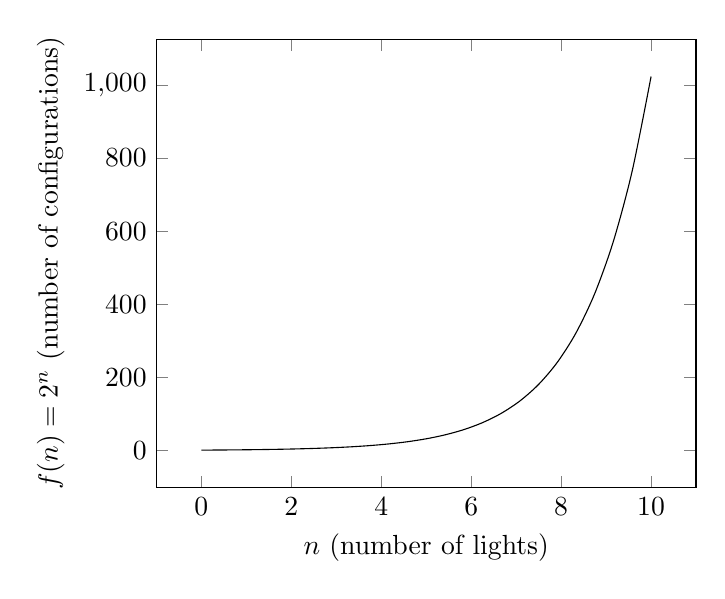
\begin{tikzpicture}[domain=0:10,yscale=1,xscale=1,smooth]
  \begin{axis}[ 
    xlabel=$n \text{ (number of lights)}$,
    ylabel={$f(n) = 2^n \text{ (number of configurations)}$}
  ] 
    \addplot[mark=none]{2^x}; 
  \end{axis}
\end{tikzpicture} \\

Let's review. We've come up with a system that would allow us to display an English sentence using 525 lights -- recall that a set of 5 lights allowed us to display an English letter -- and then we asked the question of how many total configurations we could display with the 525 lights. We learned that this is an obscenely large number of configurations. Should we be worried at all? Is our light ssystem doomed to fail?

Actually, it's still quite alright and is a viable system of communication. We don't need to display each possible configuration, which is good, because we've just learned it's an impossible task. Instead, we generally just need to work with the configurations of lights that we care about -- the ones that help us transfer useful information.

Moreover, what we learned about exponentials above will be critical to creating systems of encryption that cannot be broken with sheer computational power alone. To help to illustrate the real-world implications of what we learned about our system of lights above, consider the following fact which we will prove later on: a random 6-character password is weak enough that it can be cracked by anyone with a laptop, but a random 12-character password is so strong that even the world's most sophisticated intelligence agencies would not even bother trying to break it.

\chapter{The Electrical Telegraph}

So far we've talked about two systems for communicating at a distance: the optical telegraph system, and the system of lights on top of Mary's house. One major limitation of both of those systems is that they rely on line of sight. What happens if it gets foggy? Or if you want to communicate across a large body of water that doesn't allow for the construction of towers along the way?

The electrical telegraph solves these problems, providing a more robust solution to long distance communication by using electricity over a wire to transmit a signal. This approach doesn't have the shortcoming of the line-of-sight approaches – the wire can snake around large mountains, treacherous deserts, and lie at the bottom of bodies of water. Moreover, it doesn't require expensive towers to be built and maintained, and wires can fairly easily be repositioned, and so a network based on the electrical telegraph turned out to be much less expensive and more flexible when compared with the optical telegraph networks. Given all the advantages of the electrical telegraph, once it became established as a viable solution, it quickly eclipsed the optical telegraph, and nowadays when someone talks about the ``telegraph'' they are almost certainly referring to the electrical telegraph. I will follow this convention, and explicitly use the phrase ``optical telegraph'' when I need to refer to the older line-of-sight Chappe technology.

The development of the electrical telegraph occurred in the first half of the 19th century, and relied on advances in battery technology and a steady progression in our ability as human beings to harness the power of electricity in increasingly sophisticated ways. Like most great inventions, the ideas behind the telegraph were developed more or less independently by more than one person.

The man who gets the majority of the credit as the father of the telegraph is Samuel Morse, a painter-turned-inventor who was born in 1792, a year after Chappe started building out his optical telegraph network in earnest. Morse was unaware of telegraphy through his early life; he painted portraits through his 30s and only in his 40s turned his attention towards electricity and the idea of creating a system of communication using electricity over a wire. He then obsessively worked on this problem until he eventually developed and popularized the dominant telegraphy system which became the standard for telegraphy for the next sixty years.

Besides Morse, the other prominent pair of inventors were Cooke and Wheatstone, who worked in England, and developed ideas independently of the American-born painter-turned-inventor. Conceptually, all of these people were on a similar track, but Morse's system had certain advantages over that of Cooke and Wheatstone, and eventually even Cooke and Wheatstone agreed that the “Morse system” was superior. [CITE]

\section{Circuits}

An electric telegraph is in essence just a very simple electrical circuit. There is a power source, a switch and a loop of wire connected to an electrical device that one would like to operate:

[DIAGRAM]

In the circuit diagram above, the power source is the battery is drawn on the left. It has positive and negative terminals, which we'll talk about in a minute. The little angled line represents a switch. If the switch is open, as it is in the diagram above, electricity does not flow through the circuit. If the switch it closed, on the other hand, then an electric current flows through this circuit:

[DIAGRAM]


\chapter{Symbols and Ciphers}

\end{document}
